\documentclass[conference]{IEEEtran}
%\IEEEoverridecommandlockouts
% The preceding line is only needed to identify funding in the first footnote. If that is unneeded, please comment it out.
\usepackage{cite}
\usepackage{amsmath,amssymb,amsfonts}
\usepackage{algorithmic}
\usepackage{graphicx}
\usepackage{textcomp}
\usepackage{xcolor}
\usepackage{cuted}
\usepackage{tikz}
\usepackage{pgfplots}
\usepackage{url}


\usetikzlibrary{calc,trees,positioning,arrows,chains,shapes.geometric,%
    decorations.pathreplacing,decorations.pathmorphing,shapes,%
    matrix,shapes.symbols}

\tikzstyle{line} = [draw, -, thick]
\tikzstyle{nodraw} = [draw, fill, circle, minimum width=0pt, inner sep=0pt]
\tikzstyle{box} = [line, rectangle, rounded corners, text centered]

\tikzset{
>=stealth',
  punktchain/.style={
    rectangle, 
    rounded corners, 
    draw=black, very thick,
    text width=2em, 
    minimum height=3em, 
    text centered, 
    on chain},
  line/.style={draw, thick, <-},
  element/.style={
    tape,
    top color=white,
    bottom color=blue!50!black!60!,
    minimum width=1em,
    draw=blue!40!black!90, very thick,
    text width=2em, 
    minimum height=3.5em, 
    text centered, 
    on chain},
  every join/.style={->, thick,shorten >=1pt},
  decoration={brace},
  tuborg/.style={decorate},
  tubnode/.style={midway, right=2pt},
}


\def\BibTeX{{\rm B\kern-.05em{\sc i\kern-.025em b}\kern-.08em
    T\kern-.1667em\lower.7ex\hbox{E}\kern-.125emX}}
\newcommand*\Laplace{\mathop{}\!\mathbin\bigtriangleup}
\begin{document}

\title{Combining checkpointing and data compression to accelerate
  adjoint-based optimization problems}

\author{\IEEEauthorblockN{Navjot Kukreja}
\IEEEauthorblockA{%\textit{Department of Earth Science and Engineering} \\
\textit{Imperial College London}\\
London, UK \\
n.kukreja@imperial.ac.uk}
\and
\IEEEauthorblockN{Jan H\"uckelheim}
\IEEEauthorblockA{%\textit{Department of Earth Science and Engineering}\\
\textit{Imperial College London}\\
London, UK }
\and
\IEEEauthorblockN{Mathias Louboutin}
\IEEEauthorblockA{%\textit{School of Computational Science and Engineering} \\
\textit{Georgia Institute of Technology}\\
Atlanta, GA, USA\\}
%\and
%\IEEEauthorblockN{Kaiyuan Hou}
%\IEEEauthorblockA{%\textit{Department of Electrical Engineering and Computer Science} \\
%\textit{Northwestern University}\\
%Evanston, IL, USA \\
%}
%\and
%\IEEEauthorblockN{Fabio Luporini}
%\IEEEauthorblockA{%\textit{Department of Earth Science and Engineering} \\
%\textit{Imperial College London}\\
%London, UK \\
%}
\and
\IEEEauthorblockN{Paul Hovland}
\IEEEauthorblockA{%\textit{Mathematics and Computer Science Division} \\
\textit{Argonne National Laboratory}\\
Lemont, IL, USA \\
}
\and
\IEEEauthorblockN{Gerard Gorman}
\IEEEauthorblockA{%\textit{Department of Earth Science and Engineering}\\
\textit{Imperial College London}\\
London, UK }
}

\maketitle

\begin{abstract}
Seismic inversion and imaging are adjoint-based optimization problems that processes up to terabytes of data, regularly exceeding the memory
capacity of available computers. Data compression is an effective strategy to
reduce this memory requirement by a certain factor, particularly if some loss in
accuracy is acceptable. A popular alternative is checkpointing, where data is
stored at selected points in time, and values at other times are recomputed as
needed from the last stored state.  This allows arbitrarily large adjoint
computations with limited memory, at the cost of additional recomputations.

In this paper we combine compression and checkpointing for the first
time to compute a realistic seismic inversion. The combination of
checkpointing and compression allows
larger adjoint computations compared to using only compression, and
reduces the recomputation overhead significantly compared to using only checkpointing.
\end{abstract}

\begin{IEEEkeywords}
Checkpointing, compression, adjoints, inversion, seismic
\end{IEEEkeywords}

\section{Introduction}

\subsection{Adjoint-based optimization}
Adjoint-based optimization problems typically consist of a simulation
that is run forward in simulation time, producing data that is used in
reverse order by a subsequent adjoint computation that is run
backwards in simulation time.  Figure~\ref{fig:dataflow} shows the
resulting data flow. Besides seismic inversion, many important
numerical problems in science and engineering use adjoints and follow
the same pattern. 

Since the data for each of the computed timesteps in the forward
simulation will be used later in the adjoint computation, it would be
prudent to store it in memory until it is required again, if the required amount
of memory is indeed available. However, the total size of this data
can often run into tens of terabytes and the management of this data
becomes a problem in itself. This data management problem is the
subject of this paper. 

\begin{figure}
\begin{center}
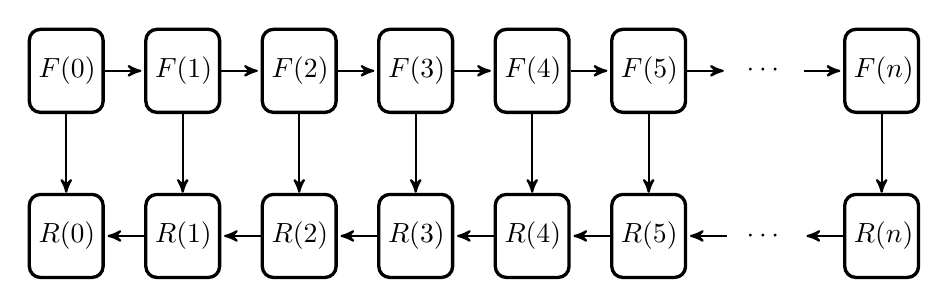
\begin{tikzpicture}
  [node distance=.5cm,
  start chain=1 going right,start chain=2 going left]
     \node[punktchain, join, on chain=1] (t1) {$F(0)$};
     \node[punktchain, join, on chain=1] (t2)      {$F(1)$};
     \node[punktchain, join, on chain=1] (t3)      {$F(2)$};
     \node[punktchain, join, on chain=1] (t4) {$F(3)$};
     \node[punktchain, join, on chain=1] (t5) {$F(4)$};
     \node[punktchain, join, on chain=1] (t6) {$F(5)$};
     \node[punktchain, join, draw=none, on chain=1] (ellipsis1) {$\cdots$};
     \node[punktchain, join, on chain=1] (tn) {$F(n)$};

\node[punktchain, below=1cm of tn, on chain=2] (atn) {$R(n)$};
\node[punktchain, join, draw=none, on chain=2] (ellipsis2) {$\cdots$};
     \node[punktchain, join, on chain=2] (at6)      {$R(5)$};
     \node[punktchain, join, on chain=2] (at5)      {$R(4)$};
     \node[punktchain, join, on chain=2] (at4) {$R(3)$};
     \node[punktchain, join, on chain=2] (at3) {$R(2)$};
     \node[punktchain, join, on chain=2] (at2) {$R(1)$};
     \node[punktchain, join, on chain=2] (at1) {$R(0)$};

\draw[|-,-|,->, thick,] (t1.south) |-+(0,-1em)-| (at1.north);
\draw[|-,-|,->, thick,] (t2.south) |-+(0,-1em)-| (at2.north);
\draw[|-,-|,->, thick,] (t3.south) |-+(0,-1em)-| (at3.north);
\draw[|-,-|,->, thick,] (t4.south) |-+(0,-1em)-| (at4.north);
\draw[|-,-|,->, thick,] (t5.south) |-+(0,-1em)-| (at5.north);
\draw[|-,-|,->, thick,] (t6.south) |-+(0,-1em)-| (at6.north);
\draw[|-,-|,->, thick,] (tn.south) |-+(0,-1em)-| (atn.north);
  \end{tikzpicture}
\end{center}
\caption{The dataflow pattern that is typical of adjoint-based optimization problems}
\label{fig:dataflow}
\end{figure}

\subsection{Example adjoint problem: Seismic inversion}
Seismic inversion typically involves the simulation of the propagation
of seismic waves through the earth's subsurface, followed by a
comparison with data from field measurements. The model of the
subsurface is iteratively improved by minimizing the misfit between
simulated data and field measurement in an adjoint optimization
problem.  Figure~\ref{fig:offshore_survey} shows the setup of the
field experiment that produces the measured
data~\cite{plessix2006review}. 


The data collected in an offshore survey typically consists of a
number of ``shots'' - each of these shots corresponding to different
locations of sources and receivers. As a loose analogy with machine
learning, these correspond to different data points. Since the
gradient computation over a single shot is complex enough that a
single shot can occupy a complete node for $~10^1-10^2$ minutes, the gradient is computed for each of these
shots independently and then collated across all the shots to form a
single update that is used to update the model. It might be evident
here that the processing across shots is easy to parallelise since it
requires a small amount of communication followed by a relatively long
period of independent computation as part of a single iteration of the
optimisation. Since the number of shots is typically of the order of
$10^4$, this offers ample opportunity to fill up a large cluster with
computation, even if an individual shot is only processed on a single
node of the cluster at a time. Hence, it might be worthy to note that
even though this paper focusses on a single gradient evaluation for a
single shot, the overall problem involves carrying out $~10^5$ such
evaluations and is typically run on large clusters for non-trivial
amounts of time.

The first part of seismic inversion, i.e. the simulation of seismic
wave propagation through the earth's subsurface is typically done
using a finite-difference solver and is called the ``forward problem''
in the context of inversion. Looking at this part in isolation, the
data flow here looks like the one shown in
figure~\ref{fig:dataflowfw}. This illustration assumes a first-order
time-stepper, i.e. the computation of each timestep only depends on
the previous timestep. In such a scenario, only two timesteps need to
be kept in memory - the last computed step and the one currently being
computed. In case of an n-th order time-stepper, $(n+1)$ timesteps
need to be kept in memory at any one time. Hence, the memory
requirements of the forward problem can remain constant, regardless of
the number of timesteps the simulation may be run for.

\begin{figure*}
\begin{center}
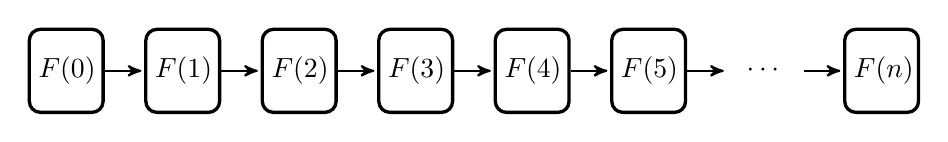
\begin{tikzpicture}
  [node distance=.5cm,
  start chain=1 going right,start chain=2 going left]
     \node[punktchain, join, on chain=1] (t1) {$F(0)$};
     \node[punktchain, join, on chain=1] (t2)      {$F(1)$};
     \node[punktchain, join, on chain=1] (t3)      {$F(2)$};
     \node[punktchain, join, on chain=1] (t4) {$F(3)$};
     \node[punktchain, join, on chain=1] (t5) {$F(4)$};
     \node[punktchain, join, on chain=1] (t6) {$F(5)$};
     \node[punktchain, join, draw=none, on chain=1] (ellipsis1) {$\cdots$};
     \node[punktchain, join, on chain=1] (tn) {$F(n)$};

  \end{tikzpicture}
\end{center}
\caption{The dataflow pattern typical of a forward-only
  simulation. Boxes represent data and arrows represent computation.}
\label{fig:dataflowfw}
\end{figure*}


TODO remove contractions

\subsection{Memory requirements}
A number of strategies are regularly employed to deal with this
enormous volume of data - the simplest of these being to store it to a
disk, to be read later by the adjoint pass in reverse order. However,
typically the computation to be done on this data in the adjoint phase
takes much less time than the time taken to read it from the disk,
reading from the disk becomes the bottleneck for most practical cases,
rendering this method, although possibly the simplest, also the
slowest of the possible alternatives. Seeing this from the perspective
where thousands of such computations might be running in parallel on a
single cluster (for different shots), the network bandwidth might
restrict the use of a network storage further, hence only node-local disks
may be suitable for this strategy. 

Domain decomposition, where a single shot may be distributed across more
than one node, is often used not only to distribute the computational
workload across more processors, but also to utilize the large amount of memory
available in distributed systems. While this strategy is very powerful, the
number of compute nodes and therefore the amount of memory that can be used
efficiently is limited, for example by communication overheads that start to
dominate as the domain is split into increasingly small
pieces~\cite{virieux2009seismic}. Secondly, this strategy can lead to
a wastage of resources and sometimes a longer time-to-solution for a
given inversion problem using a given number of nodes, especially when
the number of nodes is less than the number of shots. For example, a
problem setup that requires only 10\% more memory than is available on
a single node might not be a good candidate for domain decomposition
over multiple nodes. Lastly, this method is even less applicable on
cloud-based setups since it can be drastically more complicated
to setup and slower due to the communication.


Another common strategy in seismic inversion is to only store values
at the boundaries of the domain at each timestep, and reconstruct the
rest of the wavefield when
required~\cite{clapp2009reverse,yang2014rtm} with time reversal of the
wave equation. However, this method is not applicable for wave
equations that are not time reversible when for example physical
attenuation is included.

Checkpointing is yet another strategy to reduce the memory
overhead. Only a subset of the timesteps during the forward pass is
stored (and the rest discarded). The discarded data is recomputed when
needed by restarting the forward pass from the last available stored
state. We discuss this strategy in section~\ref{revolve}.

Another strategy commonly employed to reduce the memory footprint of
such applications is data compression. This is discussed in
section~\ref{compression}. 

In this paper, we extend the previous studies by \emph{combining} checkpointing
and compression. This is obviously useful when the data does not fit in the
available memory even after compression, for example for very large adjoint
problems, or for problems where the required accuracy limits the achievable
compression ratios.

Compared to the use of only checkpointing without compression, this
combined method often improves performance. This is a consequence of
the reduced size of stored timesteps, allowing more timesteps to be
stored during the forward computation. This in turn reduces the amount
of recomputation that needs to be performed. On the other hand, the
compression and decompression itself takes time. The answer to the
question ``does compression pay off?'', depends on a number of factors including - available
memory, the required precision, the time taken to compress and
decompress, and the achieved compression factors, and various problem specific
parameters like computational intensity of the kernel involved in the
forward and adjoint computations, and the number of timesteps.

Hence, the answer to the compression question depends not only on the
problem one is solving (within seismic inversion, there are numerous
variations of the wave equation that may be solved), but also the
hardware specifics of the machine on which it is being solved. In
fact, as we will see in section TODO, the answer might even change
during the solution process of an individual problem. This brings up
the need to be able to predict whether compression would pay off in a
given scenario, without incurring significant overheads in answering
this question. In this paper, we present the use of a performance
model to answer that question.

\subsection{Summary of contributions}
\begin{itemize}
\item Study the use of different compression algorithms to seismic
  data including 6 lossless and the two most popular lossy compression
  algorithms for floating point data. 
\item Study the compressibility behaviour of seismic data in terms of
  compression factors and compression and decompression times under
  these algorithms
\item Study the performance model for Revolve alone, that takes into
  account time taken to read and write checkpoints
\item An online performance model to predict whether compression would speed up
  an optimization problem
\end{itemize}


\section{Compression algorithms}



Data compression is increasingly used to reduce the memory footprint of
scientific applications. General purpose data compression algorithms like Zlib
(which is a part of gzip)~\cite{deutsch1996zlib}, and compression algorithms for
video and image data such as JPEG-2000~\cite{skodras2001jpeg} have been
presented in previous work. More recently, special purpose compression
algorithms for floating-point scientific data have been developed, such as ZFP
or SZ~\cite{lindstrom2014fixed,di2018efficient}.

Lossless algorithms guarantee that the exact original data can be recovered
during decompression, whereas lossy algorithms introduce an error, but often
guarantee that the error does not exceed certain absolute or relative error
metrics. Typically, lossy compression is more effective in reducing the data
size. Most popular compression packages offer various settings that allow a
tradeoff between compression ratio, accuracy, and compression and decompression
time.

Another comonly-observed difference between lossless and lossy
compression algorithms is that lossless compression algorithms tend to
interpret all data as one-dimensional series only while SZ and ZFP,
being designed for scientific data, tend to take the dimensionality
into account directly. This makes a difference in the case of a
wavefield, for example, where the data to be compressed corresponds to
a smoothly varying function in (two or) three dimensions and
interpreting this three-dimensional data as one-dimensional would
completely miss the smoothness and predictability of the data values.

It is worth noting that another data reduction strategy is to typecast values
into a lower precision format, for example, from double precision to single
precision. This can be seen as a computationally cheap lossy compression
algorithm with a compression ratio of $2$.

Perhaps counterintuitively, compression can not only reduce the memory
footprint, but also speed up an application. Previous work has observed that the
compression and decompression time can be less than the time saved from the
reduction in data that needs to be communicated across MPI nodes or between a
GPU and a host computer~\cite{gpu-compression}.

One way of using compression in adjoint-based methods is to compress
all the timesteps during the forward pass. If the compression ratio is
sufficient to fit the entire data in memory, this enables solving an
adjoint-based optimisation problem without resorting to any of the
other techniques previously discussed here. Specifically, compression
serves as an \emph{alternate strategy} to checkpointing in this
scenario. Previous work has discussed this in the context of
computational fluid dynamics~\cite{cyr2015towards,marin2016large} and seismic
inversion using compression algorithms specifically designed for
the respective applications~\cite{dalmau2014lossy,boehm2016wavefield}. 

Since the time spent on compressing and decompressing data is often
non-negligible, this raises the question whether the computational
time is better spent on this compression and decompression, or on the
recomputation involved in the more traditional checkpointing
approach. This question was previously answered to a limited extent
for the above scenario where compression is an alternative to
checkpointing, in a specific application~\cite{cyr2015towards}. We discuss
that in section TODO. 

\subsection{Lossless}
We use the python package \emph{blosc}~\cite{blosc}, which includes implementations for
six different lossless compression algorithms, namely ZLIB, ZSTD, BLOSCLZ,
LZ4, LZ4HC and Snappy. All these algorithms look at the data as a one-dimensional stream of bits
and at least the blosc implementations have a limit on the size of the one-dimensional array that
can be compressed in one call. Therefore we use the python package \emph{blosc-pack}, which is
a wrapper over the blosc library, to implement \emph{chunking}, i.e. breaking up the stream into
chunks of a chosen size, which are compressed one at a time. 

\subsection{Lossy}
\subsubsection{ZFP}
We use the lossy compression package ZFP~\cite{lindstrom2014fixed} developed in
C. To use ZFP from python, we developed a python wrapper for the reference
implementation of ZFP \footnote{To be released open source on publication}.

ZFP supports three compression modes, namely fixed-tolerance, fixed-precision
and fixed-rate. The fixed-tolerance mode limits the absolute error, while the
fixed-precision mode limits the error as a ratio of the range of values in the array to be compressed.
The fixed-rate mode achieves a guaranteed compression ratio requested by the
user, but does not provide any bounds on accuracy loss.


\subsection{SZ}
SZ~\cite{di2018efficient} is a more recently developed compression library, also focussed on lossy compression
of floating-point scientific data, also developed in C. We also wrote a python wrapper for the reference
implementation of SZ to use it as part of our benchmark suite. \footnote{Also to be released open source
upon publication}

SZ supports four compression modes, namely absolute error mode, which, similar to ZFP's fixed-tolerance
mode, allows the user to control the maximum pointwise error in absolute values. The relative ratio mode 
of SZ allows the user to specify a maximum error as a ratio of the range of values in the array, which is
effectively similar to ZFP's fixed-precision mode but not exactly. SZ has two other modes that are missing 
in ZFP, namely pointwise relative error and pointwise SNR mode. In the pointwise relative error mode, the user
can provide a relative error ratio and SZ will ensure that the error at each point is within that ratio, considering
its absolute value. In the pointwise SNR mode, the user provides a signal-to-noise ratio value that SZ respects
at each point.

\subsection{Combining lossy and lossless compression}
Another approach we attempted is a combination of lossy and lossless compression 
schemes to achieve an overall lossless compression scheme. Here, the array is first compressed using a 
lossy compression scheme, following which the errors incurred by this lossy scheme are passed on to a 
lossless scheme for compression. The idea is that the distribution of errors incurred by a lossy compression
algorithm might make it more favourable for lossless compression than the original array.

\section{Revolve: Performance model}
\label{sec:revolve}
Checkpointing is a commonly used strategy to reduce the memory footprint
of adjoint problems. Here, depending on the memory available, some timesteps
computed in the forward pass are stored, while others are discarded. The ones
that were discarded are later recomputed by rerunning the forward pass from
the last stored checkpoint. 
The Revolve algorithm~\cite{griewank2000algorithm} provides an
answer to the question of which timesteps should be stored and which
states should be recomputed to minimize the total amount of
recomputation work. Other authors have subsequently developed
extensions to Revolve that are optimal under different
assumptions~\cite{stumm2009multistage,
wang2009minimal,aupy2016optimal,schanen2016asynchronous, aupy2017periodicity}. Previous
work has applied checkpointing to seismic imaging and inversion
problems~\cite{symes2007reverse, datta2018asynchronous}.


In this section, we build on the ideas introduced in \cite{stumm2009multistage} to build a performance model that can be used to predict the runtime of an adjoint computation that uses the Revolve checkpointing strategy. 
We call the time taken by a single forward computational step $C_F$
and correspondingly, the time taken by a single backward step $C_R$. For a simulation with $\mathbf{N}$ timesteps, the minimum wall time required
for the full forward-adjoint evaluation is given by
\begin{equation}
T_N = \mathbf{C_F} \cdot \mathbf{N} + \mathbf{C_R} \cdot \mathbf{N}
\end{equation}
If the size of a single timestep in memory is given by $\mathbf{S}$, this
requires a memory of at least size $\mathbf{S} \cdot \mathbf{N}$. If sufficient memory
is available, no checkpointing or compression is needed.

If the memory is smaller than $\mathbf{S} \cdot \mathbf{N}$, Revolve provides
a strategy to solve for the adjoint field by storing a subset of the $\mathbf{N}$ total checkpoints
and recompute the remaining ones. The overhead introduced by this method can be broken down into
the recomputation overhead $\mathbf{O}_R$ and the storage overhead $\mathbf{O}_S$. The recomputation
overhead is the amount of time spent in recomputation, given by
\begin{equation}
\mathbf{O}_R(N, M) = p(N, M) \cdot \mathbf{C_F},
\end{equation}
where $p(N, M)$ is the minimum number of recomputed steps from \cite{griewank2000algorithm}, reproduced
here in equation \ref{eqn:recompute}.
\begin{figure*}
\begin{equation}
p(N, M) = \begin{cases}
      N(N-1) /2, & \text{if}\ M=1 \\
      \min\limits_{1<=\widetilde{N}<=N} \{\widetilde{N} + p(\widetilde{N}, M) + p(N-\widetilde{N}, M-1)\}, & \text{if}\ M>1
    \end{cases}
    \label{eqn:recompute}
\end{equation}
\end{figure*}
In equation \ref{eqn:recompute}, M is the number of checkpoints that can be
stored in memory. Note that for $M >=N$, $\mathbf{O}_R$ would be zero. For $M <
N$, $\mathbf{O}_R$ grows rapidly as M is reduced relative to N. 

In an ideal implementation, the storage overhead $\mathbf{O}_S$ might be zero, since the computation could
be done ``in-place'', but in practice, checkpoints are generally stored in a separate section of memory and they
need to be transferred to a ``computational'' section of the memory where the computation is performed, and then
the results copied back to the checkpointing memory. This copying is a common feature of checkpointing
implementations, and might pose a non-trivial overhead when the
computation involved in a single timestep is not very large. 
This storage overhead is given by:
\begin{equation}
\mathbf{O}_{SR}(N, M) = \mathbf{W}(N, M) \cdot \frac{\mathbf{S}}{\mathbf{B}} +
\mathbf{N} \cdot \frac{\mathbf{S}}{\mathbf{B}}
\label{eqn:storage}
\end{equation}
where $\mathbf{W}$ is the total number of times Revolve writes
checkpoints for a single run, $ \mathbf{N}$ is the number of times
checkpoints are read, and $\mathbf{B}$ is the bandwidth at which these
copies happen. The total time to solution becomes
\begin{equation}
T_R = \mathbf{C_F} \cdot \mathbf{N} + \mathbf{C_R} \cdot \mathbf{N} + \mathbf{O}_R(N, M) +
\mathbf{O}_{SR}(N, M)
\end{equation} 

\section{Performance model including compression}

By using compression, the size of each checkpoint is reduced and therefore the
number of checkpoints available is increased ($M$ in equation
\ref{eqn:recompute}). This reduces the recomputation overhead $\mathbf{O}_R$,
while at the same time adding overheads related to compression and decompression
in $\mathbf{O}_S$.
To be beneficial, the reduction in $\mathbf{O}_R$ must offset the increase in 
$\mathbf{O}_{SR}$, leading to an overall decrease in the time to solution $T$.

Our performance model assumes
 that the compression algorithm behaves uniformly
across the different time steps of the simulation, i.e. that we get the same compression ratio, compression time and 
decompression time, no matter which of the $N$ possible checkpoints we try to compress/decompress. The storage overhead
now becomes
\begin{equation}
\begin{split}
\mathbf{O}_{SR}(N, M) = &\mathbf{W}(N, M \cdot F) \cdot \left(\frac{\mathbf{S}}{\mathbf{F}
  \cdot \mathbf{B}} + t_c\right) +\\&\mathbf{N} \cdot
\left(\frac{\mathbf{S}}{\mathbf{F} \cdot \mathbf{B}} + t_d\right)
\end{split}
\end{equation}
where $\mathbf{F}$ is the compression ratio (i.e. the ratio between the uncompressed and compressed checkpoint), and $t_c$
and $t_d$ are compression and decompression times, respectively. At the same
time, the recomputation overhead decreases
because $\mathbf{F}$ times more checkpoints are now available.

\section{Acceptable errors and convergence}
\label{sec:errors}

Our performance model is designed to be agnostic of the specific adjoint-based 
optimization problem being solved. This is because we envision its use in a generic
checkpointing runtime that manages the checkpointed execution of the optimization
problem that accepts an acceptable error tolerance as an input parameter for each
gradient evaluation and determines whether or not compression can pay off for that
iteration, and if yes, which of the available strategies is to be used. This last question 
has previously been addressed previously in literature but in more specific contexts 
\cite{kunkel2017toward, tao2018optimizing}.

One question that arises in evaluating derivatives on grids compressed (and decompressed)
using lossy compression is the numerical stability of the computed derivatives, since errors
in neighbouring points can accumulate in the derivative rather quickly, rendering the derivatives
unusable. This question was addressed for ZFP \cite{zfp-derivatives} and SZ\cite{tao2017z}
separately.

In the context of seismic inversion, it has been shown before that the precision required
in the gradient evaluation is very low in the beginning of the optimization and
accurate gradients are not needed until the optimization is close to a minimum 
\cite{van20143d, boehm2016wavefield}. This is perhaps quite intuitive since, being far
from a minimum in the beginning, a gradient pointing in the approximate direction of the
relevant minimum is sufficient to make progress. These initial iterations could use a more
aggressive lossy compression strategy to accelerate (through compression) the progress 
towards the minimum. Once the optimization is within the vicinity of the minimum, the
gradient is required at a higher accuracy to make any progress, and this performance
model can then dynamically decide to disable compression for those iterations where
a more accurate, albeit slower, gradient evaluation is preferred. 

There is also a body of work that addresses convergence guarantees of trust-region
based optimization methods in the presence of unreliable gradients. This was primarily
done for the scenario where the gradient (and sometimes the functional itself) is known
with a probability $p$.~\cite{blanchet2016convergence,cartis2017global,chen2018stochastic}
It was shown here that the convergence rate is only affected by a factor that is 
a linear function of $p$. This analytical framework could be extended to provide bounds
on the accuracy required in a particular gradient evaluation in order to guarantee a certain
convergence rate.

Both these analyses stop at the required accuracy in the gradient evaluation. This needs
to be extended to derive acceptable error tolerances in individual grid points corresponding to a specific
error bound in the overall gradient evaluation. 


\section{Problem and test case}
We use Devito~\cite{devito-api,devito-compiler} to solve forward and adjoint
wave equation problems. Devito is a domain-specific language that enables the
rapid development of finite-difference solvers from a high-level description
of partial differential equations. The simplest version of the seismic wave
equation is the acoustic isotropic wave equation defined as:
\begin{equation}
m(x)\frac{\partial^2 u(t, x)}{\partial t^2} - \Laplace u(t, x) = q(t, x),
\label{eqn:wave}
\end{equation}
where $m(x) = \frac{1}{c^2(x)}$ is the squared slowness, $c(x)$ the spatially
dependent speed of sound, $u(t, x)$ is the pressure wavefield, $\Laplace u(t, x)$ denotes the laplacian of the wavefield and $q(t, x)$ is a source term.
Some of our experiments in Section \ref{sec:results} are performed using a more accurate
and more complex version of this equation called Tilted Transverse Isotropy
(TTI)~\cite{zhang2011stable} that takes into account the anisotopic propagation of waves in the earth subsurface (directional dependency of the speed of sound). We leave the TTI equations out of this paper
for brevity. 

The solution to equation~\ref{eqn:wave} forms the forward problem. The seismic inversion problem minimizes the misfit between simulated and observed signal given by:
\begin{equation}
\min_{m} \phi_s(m) = \frac{1}{2} \left\lVert d_{sim} - d_{obs} \right\rVert_2^2.
\end{equation}

This optimization problem is usually solved using gradient based methods such as steepest descent,
where the gradient is computed using the adjoint-state method that involves
the data-flow pattern from Figure \ref{fig:dataflow}.

The values of $m(x)$ used in this work are derived from the Overthrust
model~\cite{aminzadeh1996three} over a grid of $287 \times 881 \times
881$ points, including an absorbing layer of 40 points on each
side. The grid spacing is $25m$ in space. The propagation time is
$4sec$ that corresponds to 2500 timesteps. The wave field at the final
time is shown in Figure~\ref{fig:uncompressed}. The uncompressed size
of this single time step field is just under 900MB. If one were to
store all the timesteps, this would require 2.3TB of memory.

\begin{figure}
\begin{center}
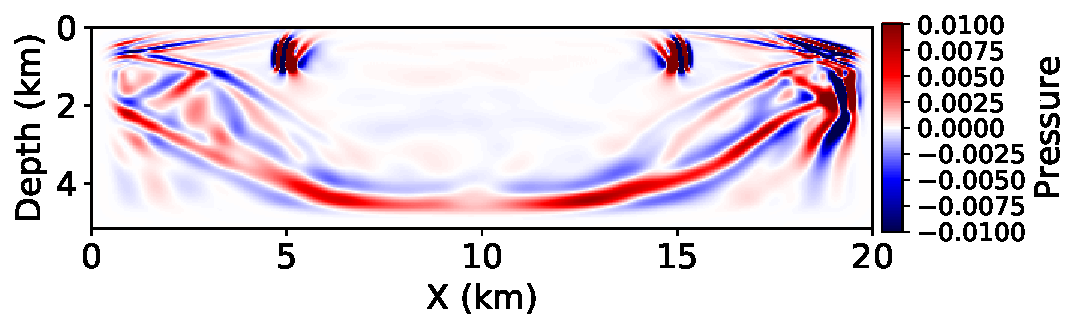
\includegraphics[width=0.8\linewidth]{images/uncompressed.pdf}
\end{center}
\caption{Cross-section of the wavefield used as a reference sample for
  compression and decompression. This field was formed after a Ricker
  wavelet source was placed at the surface of the model and the wave propagated for 2500
  timesteps. This is a vertical (x-z) cross-section of a 3D field, taken at
  the $y$ source location}
\label{fig:uncompressed}
\end{figure}

To implement Revolve with Devito, we use pyRevolve~\cite{kukreja2018high} which
is a python library to manage the execution of checkpointed adjoint computations. The performance model in
section~\ref{sec:performance_model} assumes that the implementation is similar
to pyRevolve, which stores a checkpoint by copying a portion of the operator's
working memory to the checkpointing memory and similarly loads a checkpoint by
copying from the checkpointing memory to the operator's working memory. Although
a perfect implementation of checkpointing may be able to avoid these copies, the
overhead attached to these copies can be ignored for an operator that is
sufficiently computationally intensive. However, we include the overheads in the
model to verify this assumption. 

For benchmarking we used a dual-socket
Intel(R) Xeon(R) Platinum 8180M @ 2.50 Ghz (28 cores each), henceforth
called Skylake. 

\section{Results and discussion}
\label{sec:results}

TODO add figure about evolution of compressibility 

To understand the compressibility of the data produced in a typical
wave-propagation simulation, we ran a simulation as per the setup
described in section TODO, and tried to compress every single timestep
of that simulation and noted the compression ratios achieved at every
timestep. As figure TODO shows, the initial timesteps are much easier
to compress than the later ones. This is not surprising since most
wave simulations start with the field at rest, i.e. filled with zeros.

As the wave reaches more parts of the domain, the field becomes less
compressible until it achieves a stable state when the wave has
reached most of the domain. 

If the simulation had started with the field already oscillating in a
wave, it is likely that the compressibility curve for that simulation
would be flat. 

This tells us that the compressibility of the last timestep of the
solution is representative of the worst-case compressibility and hence
we used the last timestep as our reference for comparison of
compression in the following section. 

The compression ratio achieved per unit time spent during compressing
and decompressing was seen to be highest in the fixed-tolerance mode
albeit with highly unpredictable compression ratios. Figure~\ref{fig:tolerance_cf_plot} shows compression ratios for a variety of
settings for the fixed-tolerance mode. Figure
\ref{fig:decompressed_error} shows the spatial distribution of the
error after compression and decompression, compared to the original
field, using fixed-tolerance mode.
\begin{figure}
\begin{center}
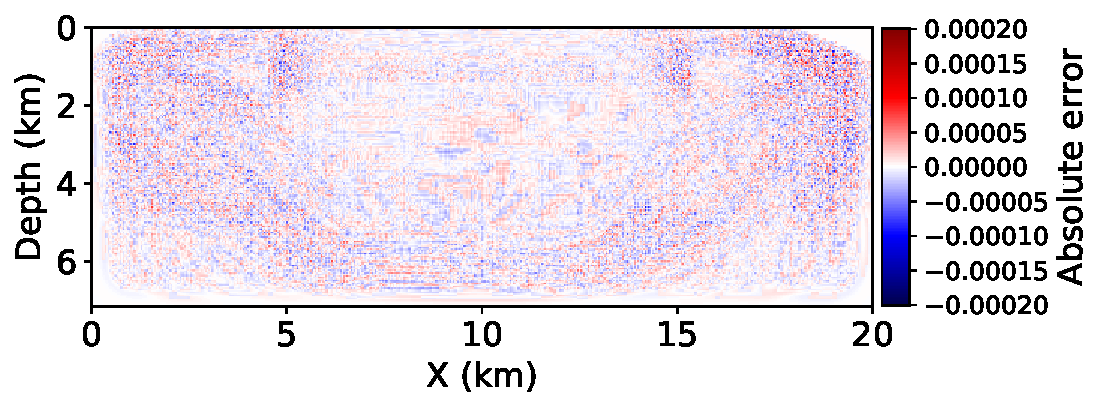
\includegraphics[width=0.8\linewidth]{images/errors.pdf}
\end{center}
\caption{Cross-section of the field that shows errors introduced
  during compression and decompression using the fixed-tolerance
  mode. It is interesting to note that the errors are more or less
  evenly distributed across the domain with only slight variations
  corresponding to the wave amplitude (from the field plot in Figure
  \ref{fig:uncompressed}. A small block-like structure characteristic of
  ZFP can be seen.}
\label{fig:decompressed_error}
\end{figure}


\begin{figure}
\begin{center}
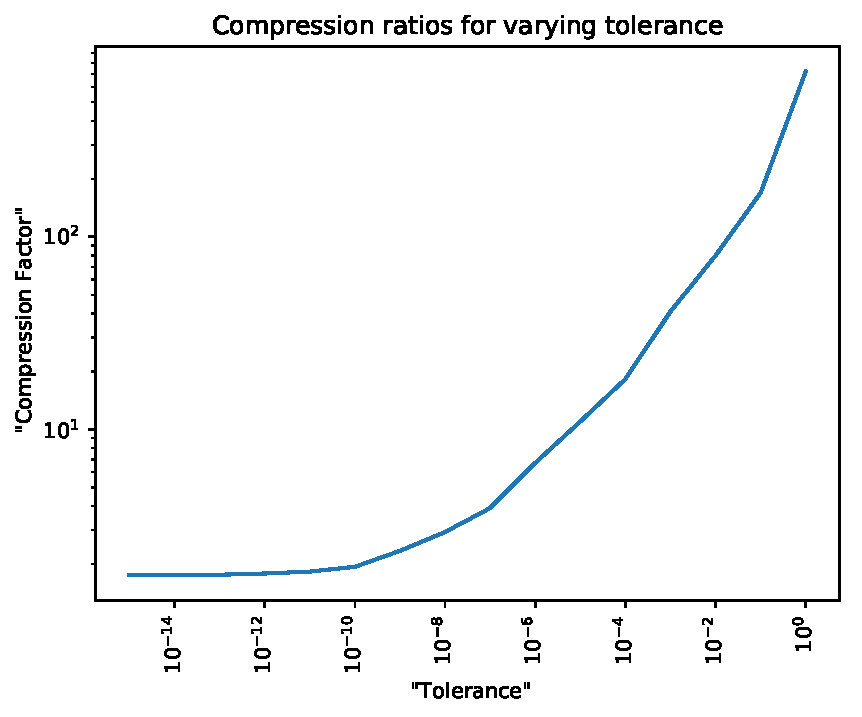
\includegraphics[width=0.9\linewidth]{images/tolerance-cf-richter.pdf}
\end{center}
\caption{Compression ratios achieved on compressing the wavefield. We
  define compression ratio as the ratio between the size of the
  uncompressed data and the compressed data. The dashed line
  represents no compression. The highlighted point corresponds to the
  setting used for the other results here unless otherwise specified.}
\label{fig:tolerance_cf_plot}
\end{figure}

TODO: -Complete forward backward run to calculate gradient and angular
difference with true gradient

We can distinguish three different scenarios, depending on the amount of
available memory.
\begin{enumerate}
\item If the memory is insufficient even with compression to store the entire
trajectory, one can either use checkpointing only, or combine checkpointing with
compression.
\item If the available memory is not sufficient to store the uncompressed
trajectory, but large enough to store the entire compressed trajectory, we study
the two possible strategies: Either use compression only, or use checkpointing
only.
\item If the available system memory is large enough to hold the entire
uncompressed trajectory, neither compression nor checkpointing is necessary.
\end{enumerate}
All three scenarios can be seen in
Figure~\ref{fig:varying_memory}. TODO elaborate on which part of the
figure shows which scenario. 
The second scenario was studied in previous work~\cite{cyr2015towards}, while
the combined method is also applicable to the first scenario, for which previous
work has only used checkpointing without compression.

We can identify a number of factors that make compression more likely to be
beneficial compared to pure checkpointing: A very small system memory size and a
large number of time steps lead to a rapidly increasing recompute factor, and
compression can substantially reduce this recompute factor. This can be seen in
Figures~\ref{fig:varying_memory} and~\ref{fig:varying_nt}.

The extent to which the recompute factor affects the overall runtime also
depends on the cost to compute each individual time step. If the compute cost
per time step is large compared to the compression and decompression cost, then
compression is also likely to be beneficial, as shown in
Figure~\ref{fig:varying_compute}. As the time per time step increases and the
compression cost becomes negligible, we observe that the ratio between the runtime
of the combined method and that of pure checkpointing is only determined by the
difference in recompute factors.

\subsection{Validation of model}
TODO write this section with a plot where theoretical prediction is
shown overlaid with real measurements

Do this for: 
- Acoustic, where compression doesn't pay off
- TTI where compression performs better than recomputation

\begin{figure}
\begin{center}
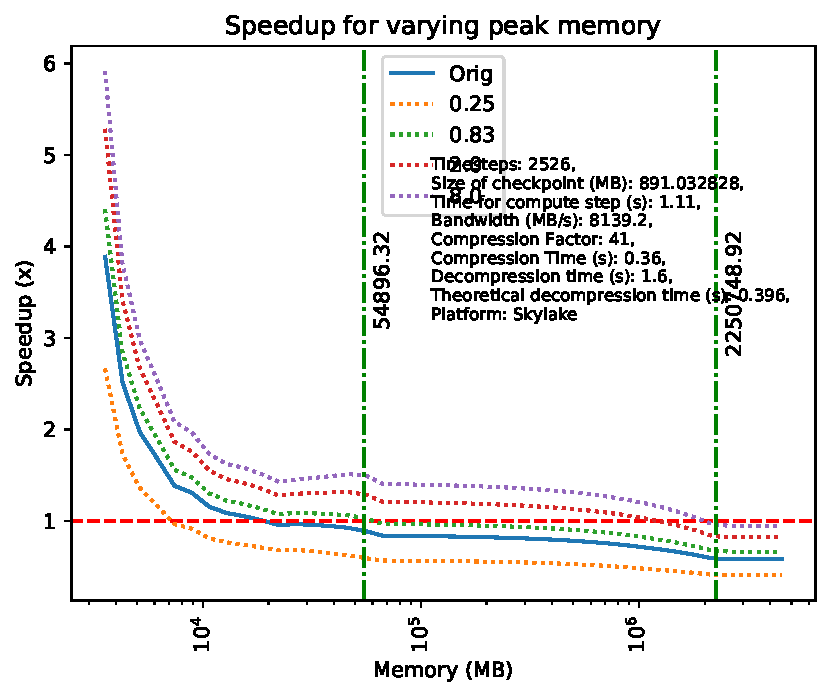
\includegraphics[width=0.9\linewidth]{images/varying-memory.pdf}
\end{center}
\caption{The speedups predicted by the performance model for varying
  memory. The baseline
(1.0) is the performance of a Revolve-only implementation under the
same conditions. The different curves represent kernels with differing
compute times (represented here as a factor of the sum of compression
and decompression times). The first vertical line at $~$ 53GB marks the
spot where the compressed wavefield can completely fit in memory and
Revolve is unnecessary if using compression. The second vertical line
at $~$ 2.2 TB marks the spot where the entire uncompressed wavefield can
fit in memory and neither Revolve nor compression is necessary. The
region to the right is where these optimisations are not necessary or
relevant. The middle region has been the subject of past studies using
compression in adjoint problems. The region to the left is the focus
of this paper.}
\label{fig:varying_memory}
\end{figure}

\begin{figure}
\begin{center}
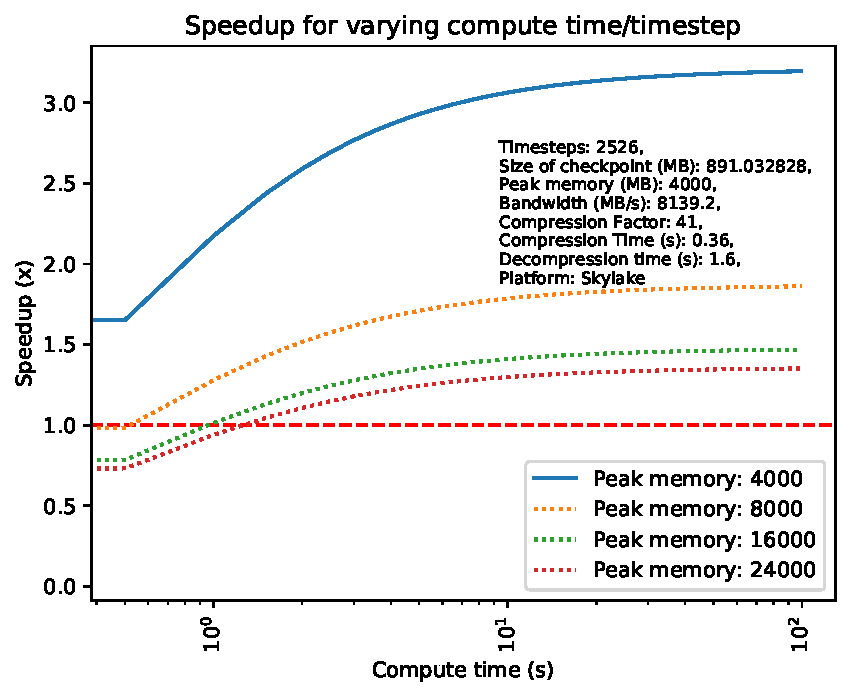
\includegraphics[width=0.9\linewidth]{images/varying-compute.pdf}
\end{center}
\caption{The speedups predicted by the performance model for varying
  compute cost. The baseline
(1.0) is the performance of a Revolve-only implementation under the
same conditions. The benefits of compression drop rapidly if the
computational cost of the kernel that generated the data is much lower
than the cost of compressing the data. For increasing computational
costs, the benefits are bounded.}
\label{fig:varying_compute}
\end{figure}

\begin{figure}
\begin{center}
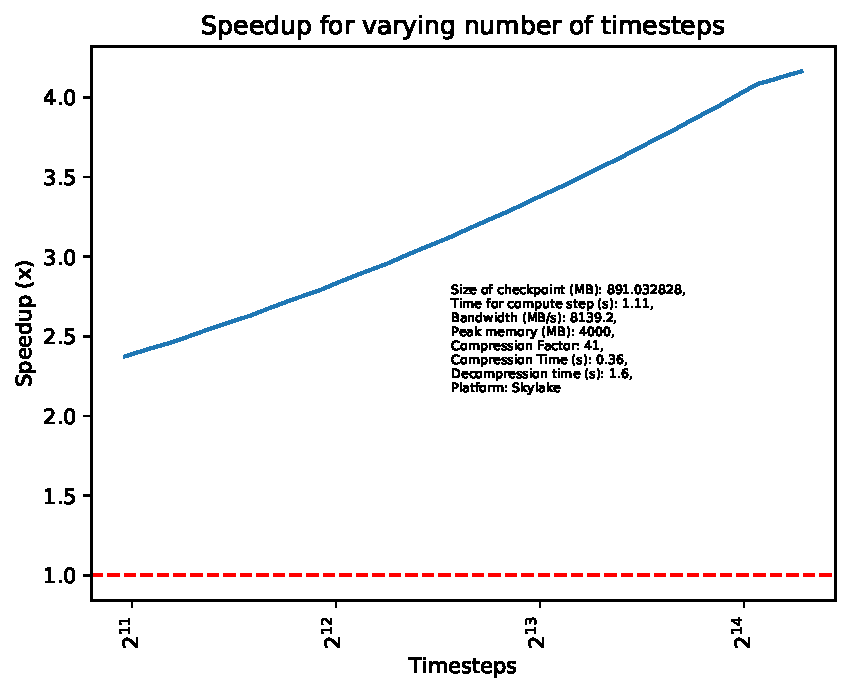
\includegraphics[width=0.9\linewidth]{images/varying-nt.pdf}
\end{center}
\caption{The speedups predicted by the performance model for varying
  number of timesteps to be reversed. The baseline
(1.0) is the performance of a Revolve-only implementation under the
same conditions. It can be seen that compression becomes more
beneficial as the number of timesteps is increased.}
\label{fig:varying_nt}
\end{figure}

\section{Conclusions and Future work}
We use lossy compression to reduce the computational overhead of
checkpointing in an adjoint computation used in seismic
inversion, a common method in seismic imaging applications whose
memory footprint commonly exceeds the available memory size in high
performance computing systems. We also developed a performance model
that computes whether or not the combination of compression and
checkpointing will outperform pure checkpointing or pure compression
in a variety of scenarios, depending on the available memory size,
computational intensity of the application, and compression ratio and
throughput of the compression algorithm. Our current result has
several limitations that we plan to address in future work:
\begin{itemize}
\item We do not discuss the accuracy of the results after decompression. This
depends on the application, compression algorithm, and affects the achievable
compression ratios. Our performance model only requires knowledge of the
compression time and ratio, and it is up to the user of this model to determine
what accuracy is needed and thus what compression ratio is realistic for their
application. TODO this is partiall addressed now. Talk about
convergence guarantees instead. 
\item ZFP only supports serial decompression. If ZFP supported
parallel decompression, our experiments would likely show a geater region in
which the combined method is faster than pure checkpointing. Furthermore, ZFP
only supports fields with up to three dimensions, while
exploiting similarities between fields at different time steps may yield a
better compression ratio. TODO update to make more relevant.
\item Our performance model is based on uniform compression ratios and
times.  However, many applications, including seismic inversion, are likely to have
initial conditions that contain little information and are easily
compressed, and the compression ratio gradually declines as the field
becomes more complex. We based our experiments on the final wave
field, which is presumably difficult to compress.
\item In comparing pure compression with pure checkpointing, we assume
that every checkpoint is compressed and decompressed. However, if the
available memory is only slightly less than the required memory, an
implementation that compresses only a subset of the checkpoints might
outperform the expectations of our model.
\item We do not discuss multi-level checkpointing, where some
checkpoints are stored on a slower, larger device. We expect
compression to be beneficial in these scenarios due to reduced data
transfer sizes.
\item TODO scheduling
\end{itemize}

\section*{Acknowledgments}
This work was funded by the Intel Parallel Computing Centre at
Imperial College London and EPSRC EP/R029423/1. 
This work was supported by the U.S. Department of Energy, Office of Science,
Office of Advanced Scientific Computing Research, Applied Mathematics and
Computer Science programs under contract number DE-AC02-06CH11357.
We would also like to acknowledge the support from the SINBAD II project and
the member organizations of the SINBAD Consortium.

We gratefully acknowledge the computing resources provided and operated by the
Joint Laboratory for System Evaluation (JLSE) at Argonne National Laboratory.

TODO Kaiyuan, Fabio, Thomas Matthews, Paul Kelly, Oana Marin

\bibliographystyle{plain}
\bibliography{compression}

\vfill
\begin{flushright}
\normalsize
\framebox{\parbox{3in}{The submitted manuscript has been created by UChicago
Argonne, LLC, Operator of Argonne National Laboratory (`Argonne'). Argonne, a
U.S. Department of Energy Office of Science laboratory, is operated under
Contract No. DE-AC02-06CH11357. The U.S. Government retains for itself, and
others acting on its behalf, a paid-up nonexclusive, irrevocable worldwide
license in said article to reproduce, prepare derivative works, distribute
copies to the public, and perform publicly and display publicly, by or on behalf
of the Government.  The Department of Energy will provide public access to these
results of federally sponsored research in accordance with the DOE Public Access
Plan.\newline \url{http://energy.gov/downloads/doe-public-access-plan}.}}
\end{flushright}

\end{document}
